\section{Modello}
\subsection{Modello concettuale}
\begin{frame}{\subsecname}
    \begin{columns}
        \begin{column}{.55\textwidth}
            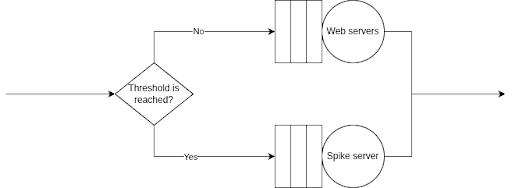
\includegraphics[width=\textwidth]{../images/modello_schematizzato.png}
            \vspace{0.7em}
            \begin{block}{Logica operativa}
                \begin{itemize}
                    \item Se \(SI < SI_{max}\) -> Web server
                    \item Se \(SI = SI_{max}\) -> Spike server
                \end{itemize}
            \end{block}
        \end{column}
        \begin{column}{.4\textwidth}
            \begin{block}{Sistema}
                \begin{itemize}
                    \item \textbf{Scheduling:} Processor sharing
                    \item \textbf{Stato del sistema:} \(S(t) = (SI(t), n_{spike}(t))\)
                    \begin{itemize}
                        \item \(SI(t)\): Utenti nel Web server
                        \item \(n_{spike}(t)\): Utenti nello Spike server
                    \end{itemize} 
                \end{itemize}
            \end{block}
        \end{column}
    \end{columns}
    
\end{frame}
\subsection{Parametri del modello}
\begin{frame}{\subsecname}
    \begin{columns}[T]
        \begin{column}{.48\textwidth}
            \begin{block}{Carico di lavoro}
                Processo iperesponenziale \\ (cv = 4)
                \begin{itemize}
                    \item \textbf{Caso Base:} \(\lambda = 6.66\) req/s
                    \item \textbf{Stress Test:} \(\lambda = \{1, 2, \ldots, 12\}\) req/s
                \end{itemize}
                \vspace{3.2em}
            \end{block}
        \end{column}
        \begin{column}{.48\textwidth}
            \begin{block}{Tempi di servizio}
                Distribuzione iperesponenziale \\ (cv = 4)
                \begin{itemize}
                    \item \textbf{Web server:} \(E[S] = 0.16 s\)
                    \item \textbf{Spike server (Base):} \(E[S] = 0.16 s\)
                    \item \textbf{Spike server (Upgrade):} \(E[S] = 0.08 s\)
                \end{itemize}
            \end{block}
        \end{column}
    \end{columns}
\end{frame}
\subsection{Modello computazionale}
\begin{frame}{\subsecname}
\end{frame}